%\title{LaTeX Portrait Poster Template}
%%%%%%%%%%%%%%%%%%%%%%%%%%%%%%%%%%%%%%%%%
% a0poster Portrait Poster
% LaTeX Template
% Version 1.0 (22/06/13)
%
% The a0poster class was created by:
% Gerlinde Kettl and Matthias Weiser (tex@kettl.de)
% 
% Adapter by Jens Buysse for Hogeschool Gent
% This template has been downloaded from:
% http://www.LaTeXTemplates.com
%
% License:
% CC BY-NC-SA 3.0 (http://creativecommons.org/licenses/by-nc-sa/3.0/)
%
%%%%%%%%%%%%%%%%%%%%%%%%%%%%%%%%%%%%%%%%%

%----------------------------------------------------------------------------------------
%	PACKAGES AND OTHER DOCUMENT CONFIGURATIONS
%----------------------------------------------------------------------------------------

\documentclass[a0,portrait]{a0poster}

\usepackage{multicol} % This is so we can have multiple columns of text side-by-side
\columnsep=100pt % This is the amount of white space between the columns in the poster
\columnseprule=3pt % This is the thickness of the black line between the columns in the poster

\usepackage[svgnames]{xcolor} % Specify colors by their 'svgnames', for a full list of all colors available see here: http://www.latextemplates.com/svgnames-colors

\usepackage{times} % Use the times font
%\usepackage{palatino} % Uncomment to use the Palatino font

\usepackage{graphicx} % Required for including images
\graphicspath{{figures/}} % Location of the graphics files
\usepackage{booktabs} % Top and bottom rules for table
\usepackage[font=small,labelfont=bf]{caption} % Required for specifying captions to tables and figures
\usepackage{amsfonts, amsmath, amsthm, amssymb} % For math fonts, symbols and environments
\usepackage{wrapfig} % Allows wrapping text around tables and figures
\usepackage[export]{adjustbox}

\begin{document}

%----------------------------------------------------------------------------------------
%	POSTER HEADER 
%----------------------------------------------------------------------------------------

% The header is divided into two boxes:
% The first is 75% wide and houses the title, subtitle, names, university/organization and contact information
% The second is 25% wide and houses a logo for your university/organization or a photo of you
% The widths of these boxes can be easily edited to accommodate your content as you see fit

\begin{minipage}[t]{0.75\linewidth}
\VeryHuge \color{HoGentAccent1} \textbf{Virtual reality als sleutel tot succesvolle
    revalidatie} \color{Black}\\ % Title

\huge \textbf{Stroobants Bruno, Lejeune Vincent, Buysse Jens}\\[0.5cm] % Author(s)
\huge Hogeschool Gent, Valentin Vaerwyckweg 1, 9000 Gent\\[0.4cm] % University/organization
\Large \texttt{bruno.stroobants.y9084@student.hogent.be} \\
\end{minipage}
%
\begin{minipage}[t]{0.25\linewidth}

\includegraphics[width=13cm,right]{figures/HOGENT_Logo_Pos_rgb.png} 

\end{minipage}

\vspace{1cm} % A bit of extra whitespace between the header and poster content

%----------------------------------------------------------------------------------------

\begin{multicols}{2} % This is how many columns your poster will be broken into, a portrait poster is generally split into 2 columns

%----------------------------------------------------------------------------------------
%	ABSTRACT
%----------------------------------------------------------------------------------------

\color{HoGentAccent1} % Navy color for the abstract

\begin{abstract}
Virtual reality is een begrip dat reeds enkele jaren in de lift zit. Maar zijn er nog verdere mogelijkheden die deze
technologie ons kan bieden dan, zoals vandaag de dag, vooral op vlak van de gaming- en entertainment-industrie
het geval is? Het zou dan ook een ultieme verrijking zijn om andere sectoren erbij te betrekken zoals bijvoorbeeld
de revalidatie. Momenteel zou virtual reality dan ook aan de vooravond kunnen staan om een ware revolutie in de
gezondheidszorg te veroorzaken.
\end{abstract}
%----------------------------------------------------------------------------------------
%	INTRODUCTION
%----------------------------------------------------------------------------------------

\color{HoGentAccent1} 
\section*{Introductie}
\color{black}
\color{black}
Wie virtual reality hoort, denkt meteen aan de talloze spellen en het plezier dat deze technologie ons
kan bieden binnen de huiskamer. Het wordt echter n`og interessanter wanneer men ook naar de mogelijkheden
daarbuiten zou kijken. Zowel op vlak van entertainment, business en ook op medisch
vlak zal VR ongetwijfeld voor grote doorbraken zorgen. De mogelijkheden ervan zijn dan ook (bijna)
eindeloos en momenteel verre van allemaal opgeklaard.

Ook in de revalidatie zou de toekomst ervan zeer groot kunnen zijn. Patiënten die zelfstandig oefeningen
dienen uit te voeren, staan vaak voor enkele uitdagingen. Zo zijn ze vaak niet gemotiveerd
om repetitieve oefeningen consistent uit te voeren. Daarnaast speelt de pijnfactor ook vaak een grote
rol bij het uitvoeren van de oefeningen.

Dit is dan ook waar virtual reality te hulp kan schieten. De patiënt zou zich meer gemotiveerd kunnen
voelen bij het uitvoeren van de oefeningen met behulp van deze technologie. Ook zou het gebruik
ervan een mogelijk pijnstillend effect op de patiënt kunnen hebben.

\begin{center}\vspace{1cm}
    
\includegraphics[width=0.5\linewidth]{synchroon}
    \captionof{figure}{\color{HoGentAccent5} Kinesitherapiepraktijk Synchroon}
\end{center}\vspace{1cm}

Gedurende dit onderzoek werd ik op vlak van kinesitherapie bijgestaan door Vincent Lejeune,
oprichter en kinesitherapeut bij Synchroon te Tienen.
%----------------------------------------------------------------------------------------
%	GEOLOGY
%----------------------------------------------------------------------------------------

\color{Black} % DarkSlateGray color for the rest of the content
\color{HoGentAccent1} 
\section*{Experimenten}
\color{black}
In kader van dit onderzoek werden er 25 fictieve patiënten tussen 19 en 85 jaar uitgenodigd om de
zelfontwikkelde VR applicatie uit te testen. Tijdens een eerste oefensessie werden er oefeningen uitgevoerd
zonder enige hulp van virtual reality, bij de tweede oefensessie kregen ze dan wel de headset
opgezet. Daarnaast werd gedurende iedere oefensessie een pijnprikkel opgewekt bij de patiënt. Na
elke sessie diende de proefpersoon enkele vragen in te vullen over hun motivatie, pijnervaring, ... Op
deze manier kon er gekeken worden naar enige verschillen in de pijnervaring en in het motivationeel
gehalte van de proefpersoon.



\color{HoGentAccent1} 

\color{black}


\begin{center}\vspace{1cm}
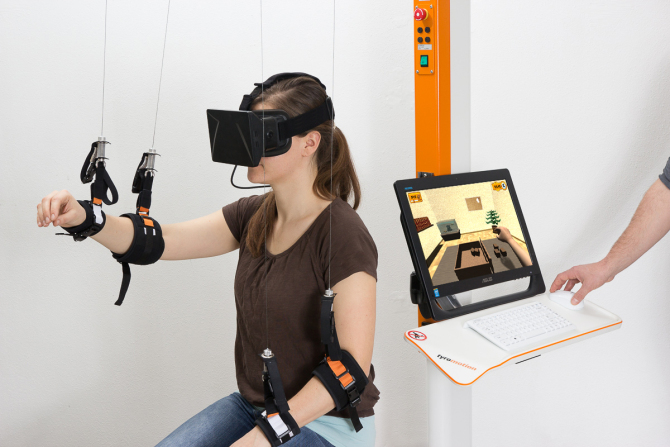
\includegraphics[width=0.8\linewidth]{poster1}
\captionof{figure}{\color{HoGentAccent5} He hasn't got shit all over him. The nose? Where'd you get the coconuts? What do you mean? We shall say 'Ni' again to you, if you do not appease us}
\end{center}\vspace{1cm}

%------------------------------------------------



\color{HoGentAccent1} 
%----------------------------------------------------------------------------------------
%	FORTHCOMING RESEARCH
%----------------------------------------------------------------------------------------
\color{HoGentAccent1} 
\section*{Toekomstig onderzoek}
\color{black}

Het zou zeker interessant zijn om dit onderwerp verder te onderzoeken aangezien de resultaten
zeker ook het potentieel van virtual reality in de revalidatie aantonen. Zo zou men bij gebruik van
gesofisticeerdere VR systemen nog tot significantere resultaten kunnen komen. Ook zou het zeer interessant
zijn om de applicatie op personen te testen met werkelijke letsels, onder begeleiding van de
kinesitherapeut.

Momenteel zijn nog niet heel veel therapeuten aan de slag gegaan met deze technologie maar
gedurende dit onderzoek werd ook duidelijk dat er zeker interesse hiervoor zou zijn en dat zij ook
de voordelen ervan bij sommige patiënten zeker inzagen.

%----------------------------------------------------------------------------------------

\end{multicols}
\end{document}